\documentclass[10pt]{beamer}
\usetheme[progressbar=frametitle]{metropolis}

\usepackage [autostyle, english = american]{csquotes}
\usepackage{amsmath}
\usepackage{amssymb}
\usepackage{bm}

\MakeOuterQuote{"}
\newcommand{\imp}[1]{\textbf{\color{cyan}#1}}

%---------------------------------------------------
% Title 

\title{Estimation of flow trajectories in a multiple lines network}
\subtitle{Case studies with \textit{transports publics de la région lausannoise} (tl) data}
\date{}
\author{Guillaume Guex \\ Romain Loup \\ François Bavaud}
\institute{University of Lausanne}

\begin{document}
	
	%------------------------------------------------------------------
	
	\maketitle
	
	%------------------------------------------------------------------
	
	\begin{frame}{Table of contents}
		\setbeamertemplate{section in toc}[sections numbered]
		\tableofcontents%[hideallsubsections]
	\end{frame}

	%------------------------------------------------------------------
	
	\section[Introduction]{Introduction}
	
	%------------------------------------------------------------------
	
	\begin{frame}{Context}
		
		The \imp{tl dataset}, used by Romain Loup for his PhD:
		
		\begin{itemize}
			\item 1 year of data (2019).
			\item 115 millions of passengers.
			\item 42 bus and subway lines.
			\item 1361 stops and 497 "superstops".
			\item Every journey data: traveling time, waiting time, embarking and disembarking passengers at each stops, etc.
		\end{itemize}
		
	\end{frame}

	%------------------------------------------------------------------
	
	\begin{frame}[fragile]{Context}
	\scriptsize
\begin{center}
\begin{verbatim}
     ##   stop_id  stop_name line_id direction order embarkment disembarkment
     ## 1 MALAD_N  Maladière       1         A     1     164558             0
     ## 2 MTOIE_E    Montoie       1         A     2     136236         12705
     ## 3 BATEL_E  Batelière       1         A     3     203045         13409
     ## 4 RTCOU_E Riant-Cour       1         A     4     156015         24909
      
     ##    stop_id  stop_name line_id direction order embarkment disembarkment
     ## 42 RTCOU_O Riant-Cour       1         R    19      23634        132201
     ## 43 BATEL_O  Batelière       1         R    20      13707        168884
     ## 44 MTOIE_O    Montoie       1         R    21       4259        128255
     ## 45 MALAD_N  Maladière       1         R    22          0        146798
\end{verbatim}

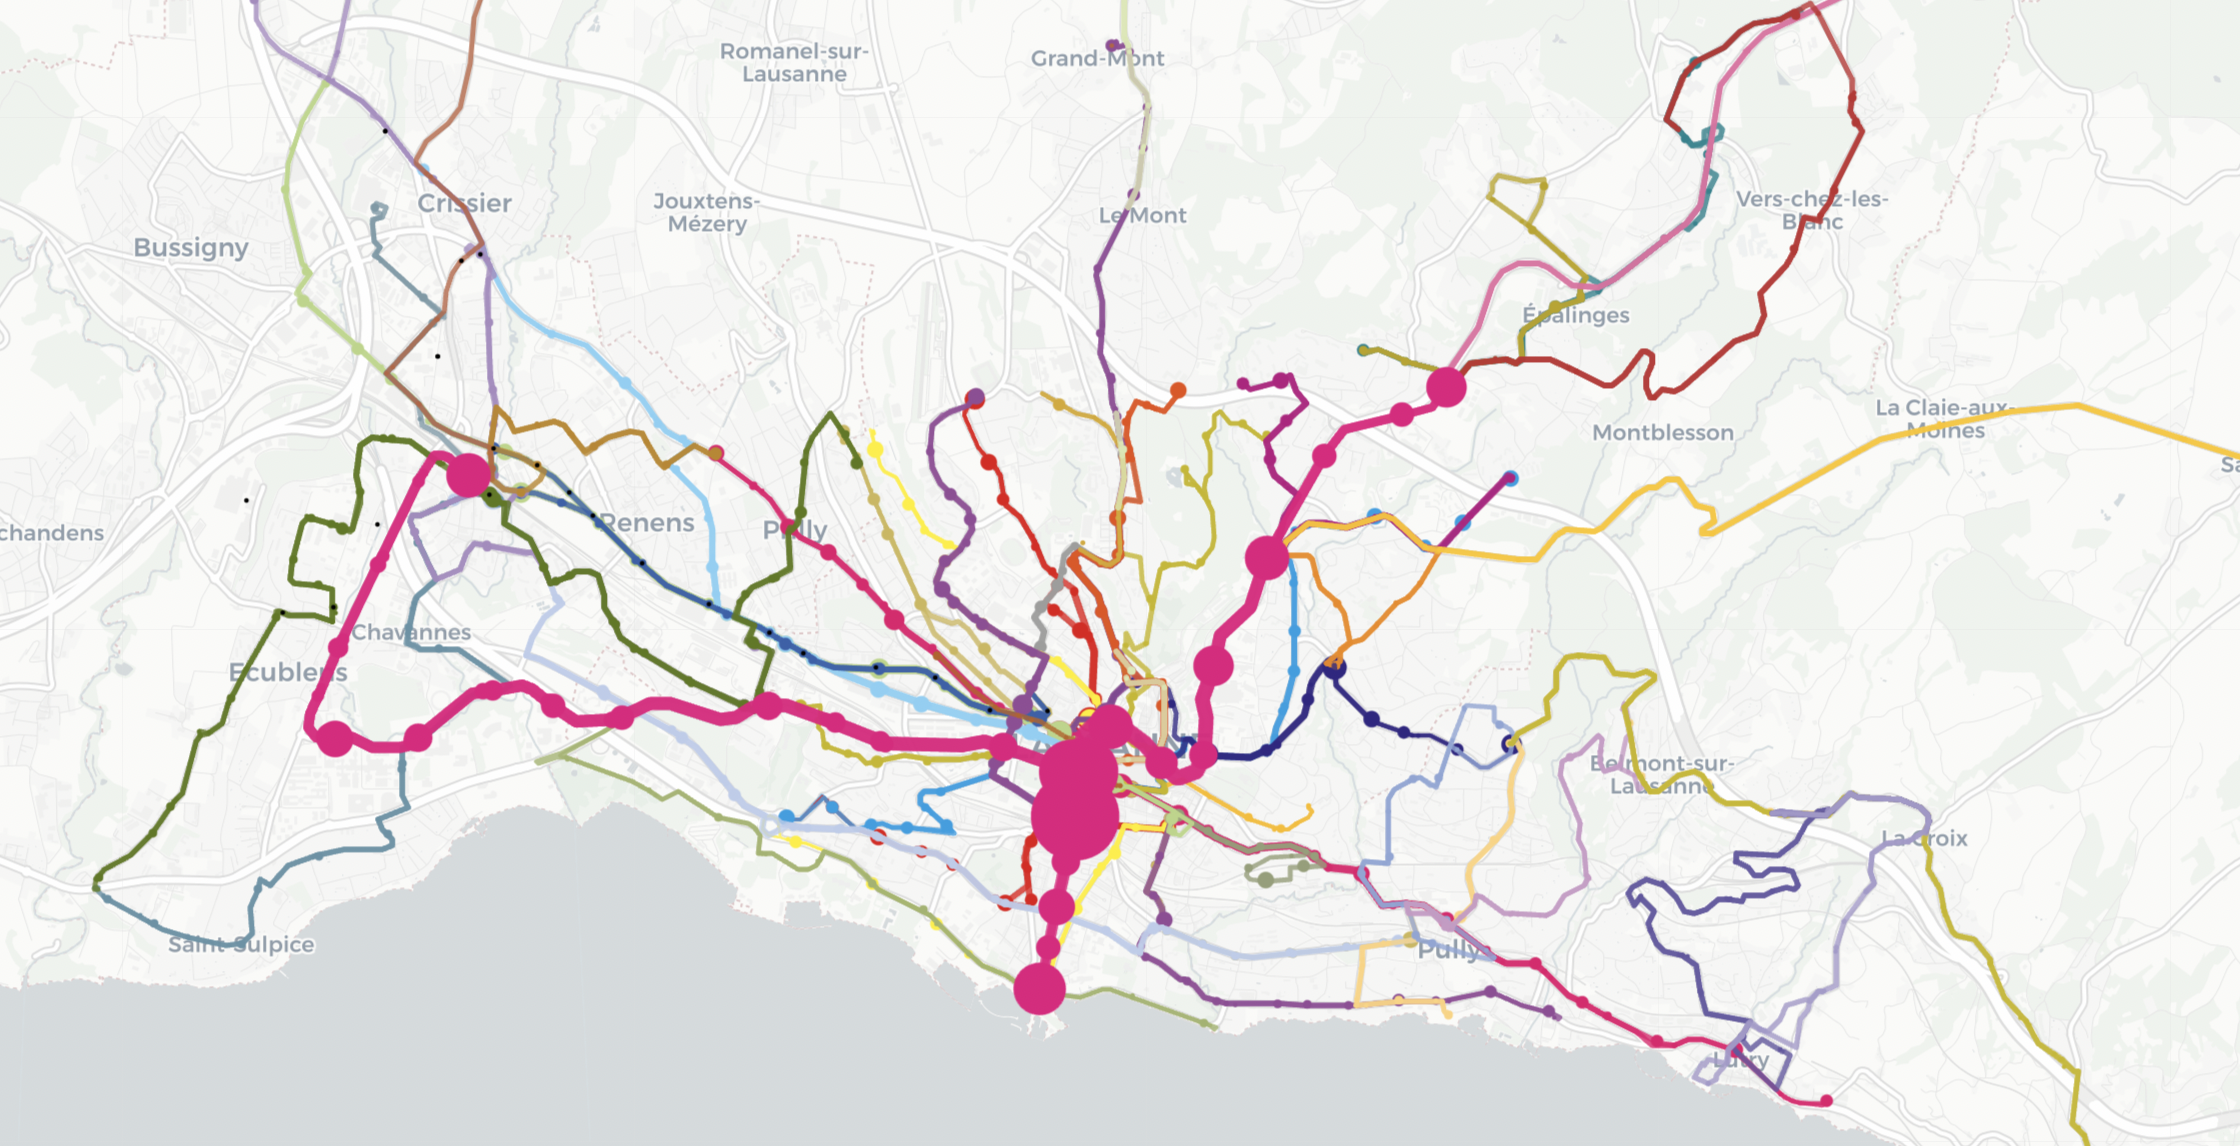
\includegraphics[width=0.7\textwidth]{img/tl_network.png}
\end{center}
	\end{frame}
	
	%------------------------------------------------------------------
	
	\begin{frame}{The multiple lines network}
		\begin{columns}
			\begin{column}{0.5\textwidth}
				Having only lines data, the structure is a \imp{disconnected oriented graph}. \linebreak
				
				In addition to \imp{line edges}, it is possible to construct \imp{transfer edges} to make the graph connected, by using, e.g.,
				\begin{itemize}
					\item Superstops names,
					\item Pedestrian time,
					\item Distance.
				\end{itemize} 
				\vspace{0.4cm}
				With transfer edges, we have a \imp{unilaterally connected graph}.
			\end{column}
			\begin{column}{0.5\textwidth} 
				\begin{center}
					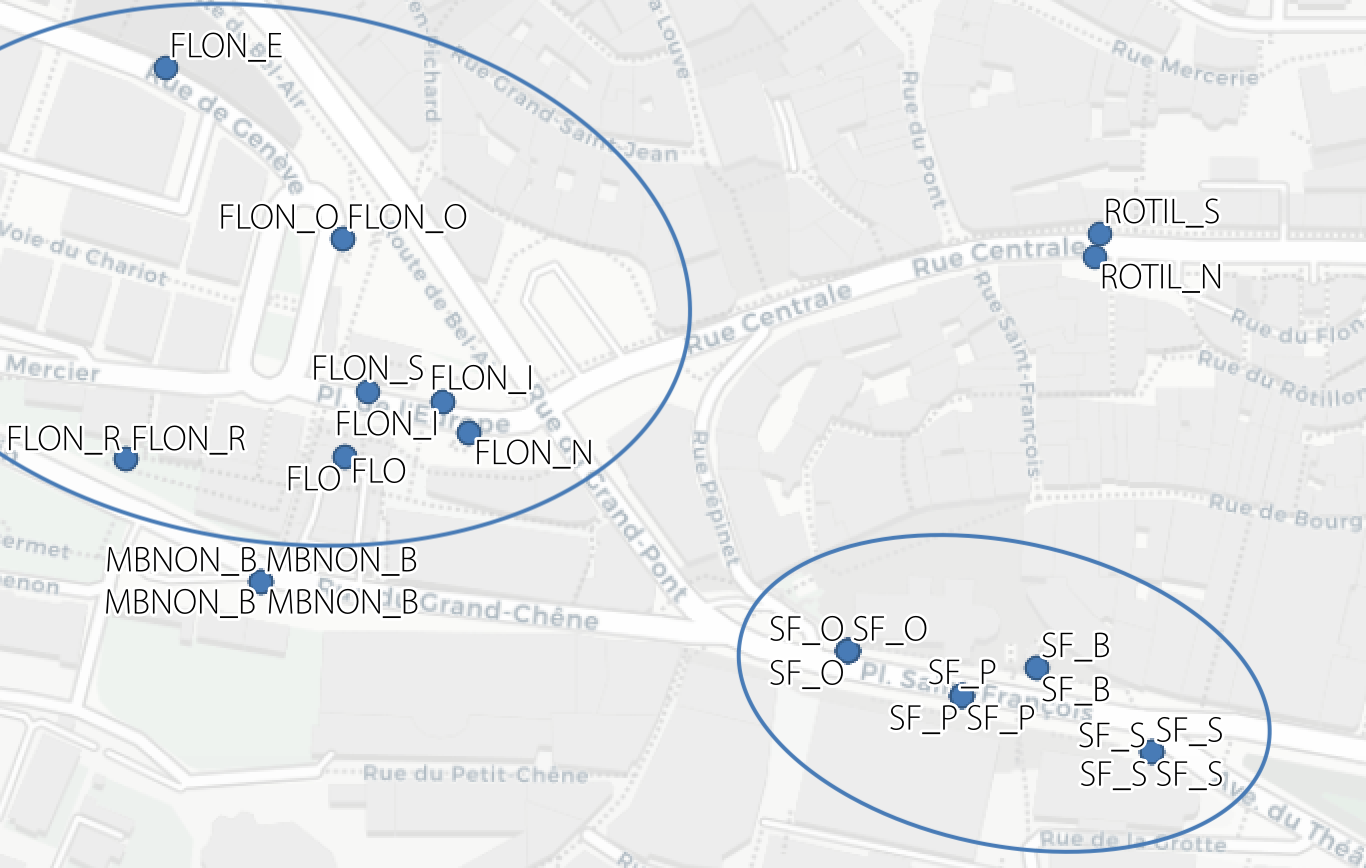
\includegraphics[width=0.8\textwidth]{img/stop_area_c.png} \\
					\vspace{0.5cm}
					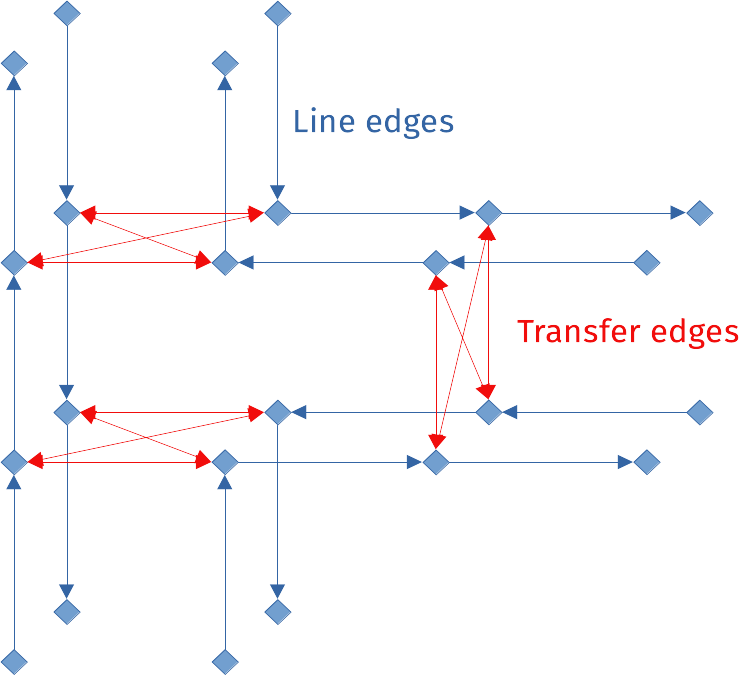
\includegraphics[width=0.7\textwidth]{img/edge_type2.png}
				\end{center}
			\end{column}
		\end{columns}
	\end{frame}
	
	%------------------------------------------------------------------

	\begin{frame}{The problematic}
		
		This dataset offers multiple axes of research. In this presentation, we will focus on one question: \vspace{0.4cm}
		
		\begin{quotation}
			\large
			Knowing \imp{(1) the network structure} and \imp{(2) the number of passengers embarking and disembarking at each stop}, can we deduce \imp{trajectories of the passengers} in the network ?
		\end{quotation}
		
	\end{frame}

	%------------------------------------------------------------------
	
	\begin{frame}{The problematic}
		
		Short answer: {\large \imp{No}}.
		
		\begin{center}
			\huge Thank you for your attention ! \\
			Questions ?
		\end{center}
		
	\end{frame}
	
	%------------------------------------------------------------------
	
	\begin{frame}{The problematic}
		
		Exact trajectories are impossible to know, but with additional hypotheses, we can \imp{estimate} them. \\
		\vspace{0.4cm}
		We will divide this problematic into two parts:
		\begin{itemize}
			\item The estimation of trajectories on a \imp{single line}.
			\item The estimation of trajectories on the \imp{multiple lines network}.
		\end{itemize}
		
	\end{frame}
	
	%------------------------------------------------------------------
	
	\section{The single line problem}
	
	%------------------------------------------------------------------
	
	\begin{frame}{Formal problem definition}
		Let a line (in one direction), which have $n$ stops. Let $\bm{\rho}_\text{in} = (\rho^\text{in}_s)$ and $\bm{\rho}_\text{out} = (\rho^\text{out}_t)$ be two vectors representing, respectively, the \imp{passengers entering and leaving lines at each stop}. \\
		\vspace{0.4cm}
		We search a $(n \times n)$ \imp{origin-destination matrix} $\mathbf{N} = (n_{st})$ where components represents
		$$
			n_{st} = \text{"\imp{the number of passengers entering line at $s$ and leaving at $t$}"}.
		$$
		These components must verify
		\begin{enumerate}
			\item $n_{st} \geq 0$,
			\item $n_{s\bullet} = \rho^\text{in}_s$,
			\item $n_{\bullet t} = \rho^\text{out}_t$.
		\end{enumerate}
		\small ($\bullet$ indicates a sum on the replaced index)
	\end{frame}
	
	%------------------------------------------------------------------
	
	\begin{frame}{Formal problem definition}
		$$
		 \mathbf{N} = \bordermatrix{
			   & \sigma^\text{out}_1 & \sigma^\text{out}_2  & \cdots & \sigma^\text{out}_{n-1} & \sigma^\text{out}_n   \cr
			\sigma^\text{in}_1 & n_{11} & n_{12} & \cdots & n_{1,n-1} & n_{1n} \cr
			\sigma^\text{in}_2 & n_{21} & n_{22} & \cdots & n_{2,n-1} & n_{2n} \cr
			\vdots & \vdots & \vdots & \ddots & \vdots & \vdots \cr
			\sigma^\text{in}_{n-1} & n_{n-1,1} & n_{n-1,2} & \cdots & n_{n-1,n-1} & n_{n-1,n} \cr
			\sigma^\text{in}_{n} & n_{n,1} & n_{n,2} & \cdots & n_{n,n-1} & n_{n,n}}
		$$
	\end{frame}
	
	%------------------------------------------------------------------
	
	\begin{frame}[allowframebreaks]{References}
		
		\bibliography{demo}
		\bibliographystyle{abbrv}
		
	\end{frame}
	
\end{document}
